\documentclass{article}
\usepackage[utf8]{inputenc}
\usepackage[english]{babel}
\usepackage{geometry}
\usepackage{amssymb}
\usepackage{amsfonts}
\usepackage{dsfont}
\usepackage{float}
\usepackage{graphicx}
\usepackage{wrapfig}
\usepackage{mathtools}
\usepackage{bbm}
\usepackage{amsthm}
\usepackage{ifthen}
\usepackage{graphicx}
\usepackage{hyperref}
\usepackage{tcolorbox}
\usepackage[ruled,vlined]{algorithm2e}
\usepackage{tikz}

\usepackage{caption}
\usepackage{subcaption}

%%%%%%%% box %%%%%%%%
\definecolor{mycolor}{rgb}{0.122, 0.435, 0.698}% Rule colour
\makeatletter
\newcommand{\mybox}[1]{%
	\setbox0=\hbox{#1}%
	\setlength{\@tempdima}{\dimexpr\wd0+13pt}%
	\begin{tcolorbox}[colframe=blue,boxrule=0.5pt,arc=4pt,
		left=6pt,right=6pt,top=6pt,bottom=6pt,boxsep=0pt,width=\@tempdima]
		#1
	\end{tcolorbox}
}
%%%%%%%%





\DeclarePairedDelimiter{\ceil}{\lceil}{\rceil}

\newcommand{\ca}[1]{\mathcal{#1}}
\newcommand{\bb}[1]{\mathbb{#1}}
\newcommand{\p}{\mathbb{P}}
\newcommand{\evento}[1]{\left\{ \textit{``#1''} \right\}}
\newcommand{\comillas}[1]{``#1''}
\newcommand{\set}[1]{\left\{#1\right\}}
\newcommand{\parent}[1]{\left(#1\right)}
\newcommand{\parentCuad}[1]{\left[#1\right]}
\newcommand{\borel}{\ca{B}(\bb{R}^d)}
\newcommand{\Rd}{\bb{R}^d}
\newcommand{\R}{\bb{R}}
\newcommand{\infNorm}[1]{||#1||_\infty}
\newcommand{\condExp}[2]{\bb{E}(#1|#2)}
\newcommand{\ind}[1]{\mathbbm{1}_{#1}}
\newcommand{\esp}[1]{\bb{E}\barras{#1}}
\newcommand{\indep}{\rotatebox[origin=c]{90}{$\models$}}
\newcommand{\pe}{$(\Omega, \ca{F}, \p)\ $}
\newcommand{\vc}[1]{\langle #1 \rangle}
\newcommand{\gb}[1]{\overline{\widehat{#1}}}
\newcommand{\barras}[1]{\left| #1 \right|}
\newcommand{\integral}{\int_{t_i}^{t_{i+1}}}
\newcommand{\ug}[1]{\widehat{\ca{U}}_{#1}}
\newcommand{\vg}[1]{\widehat{\ca{V}}_{#1}}
\newcommand{\zg}[1]{\widehat{\ca{Z}}_{#1}}
\newcommand{\norm}[1]{\left\lVert#1\right\rVert}
\newcommand{\X}{\ca{X}}
\newcommand{\xscheme}[1]{X_{t_{#1}}^{\pi}}
\newcommand{\prom}[1]{\langle #1 \rangle}


\begin{document}
%%%
% Sacar el último plot. ASD
% Rellenar las otras partes. ASD
% Terminar el uml se forma simple.
% Crear una portada.


%%% Portada %%%
\begin{titlepage}
	\centering
	{\bfseries\LARGE Universidad De Chile \par}
	\vspace{1cm}
	{\scshape\Large Facultad de Ciencias Físicas y Matemáticas \par}
	\vspace{3cm}
	{\scshape\Huge LDA con datos de Twitter \par}
	\vfill
	{\Large  Javier Castro Medina\par}

	\vfill
	{\Large Abril 2021 \par}
\end{titlepage}
%%% Portada %%%
\newpage
%%%%

\section{Análisis Exploratorio}
Para la obtención de tweets se usa la librería \texttt{twint}\footnote{\href{https://github.com/twintproject/twint}{github.com/twintproject/twint}}. Esta librería es simple de usar, permite obtener una gran cantidad de datos y almacenarlos en formato \texttt{csv} u otros. En las Figuras \ref{fig: twint_example1_informe} y \ref{fig: twint_example2_informe} se muestra, a grandes rasgos, el código que se necesita para obtener los datos utilizados en este trabajo.    


\begin{figure}[H]

	\centering
	\subfloat[]{
			\label{fig: twint_example1_informe}
			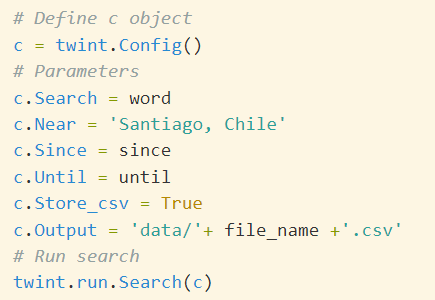
\includegraphics[scale=.5]{../imgs/twint_example1_informe.png}
	}
	%\hfill
	\subfloat[]{
			\label{fig: twint_example2_informe}
			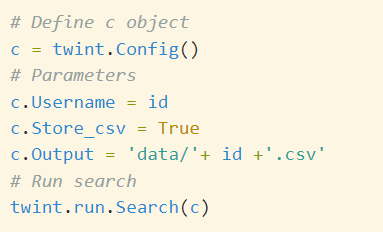
\includegraphics[scale=.5]{../imgs/twint_example2_informe.png}
	}
	\caption{A la izquierda se buscan y guardan tweets creados al rededor de Santiago entre las fechas \texttt{since} y \texttt{until} que además contengan la palabra \texttt{word}. A la derecha se obtienen y guardan los tweets de la cuenta \texttt{id}. \textbf{Scrapping tweets} es la expresión en inglés para este proceso.}
\end{figure}

En la primera parte del proyecto se realiza un proceso de adaptación a la librería \texttt{twint} y el formato de los datos que permite obtener además de un análisis superficial a los datos que obtenemos en esta fase inicial. Se decide trabajar sólo con tweets en Santiago, esto porque en tal sector hay una población más grande y por lo tanto, una probabilidad más alta de encontrar cuentas de Twitter con respecto a otros lugares. Lo que queda de esta sección se divide en dos partes, en la primera se mostrarán worclouds y en la segunda gráficos de la frecuencia de tweets diarios para distintos set de datos.

\begin{remark}
	Otra razón por la cual fijar el lugar geográfico de la obtención de tweets es disminuir la complejidad del proyecto, puede ser un aspecto a considerar en una tarea de mayor escala en la que además se tome en cuenta la variable espacial de nuestros datos.	
\end{remark}

\subsection{Wordclouds}
	Se muestran las wordclouds asociadas a tres set de tweets (o datos) distintos. Por un lado tenemos dos hitos importantes en Chile, el primero es el estallido social del $18$ de octubre del $2019$ y el segundo es el día de la mujer del $2020$. El tercero contiene los tweets que contienen la palabra \comillas{piñera} y fueron creados durante el $2020$.
	
	
	
	
   	\begin{figure}[H]
   		\centering
   		\subfloat[]{
	   		\begin{minipage}{0.33\textwidth}
	   			\centering
	   			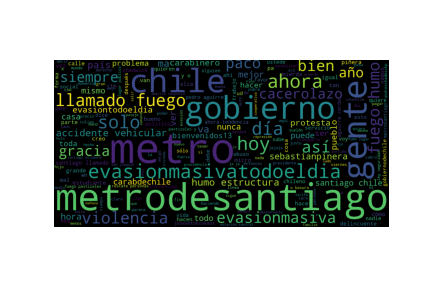
\includegraphics[width=\textwidth]{../imgs/wordcloud_santiago_estallido1.png}
	   		\end{minipage}
   			\label{fig: estallido}
   		}
   		%\hfill
   		\subfloat[]{
	   		\begin{minipage}{0.33\textwidth}
	   			\centering
	   			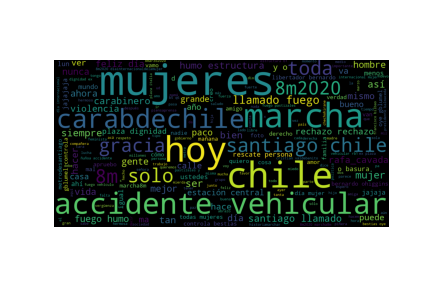
\includegraphics[width=\textwidth]{../imgs/wordcloud_santiago_8M.png}
	   		\end{minipage}
   		\label{fig: mujer}
		}
		%\vfill
		\subfloat[]{
			\begin{minipage}{0.33\textwidth}
				\centering
				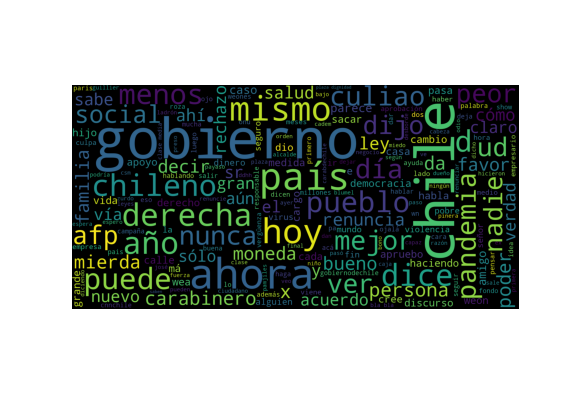
\includegraphics[width=\textwidth]{../imgs/wordcloud_santiago_pinera_2020.png}
			\end{minipage}
		\label{fig: pinera}
		
		}
		\caption{De izquierda a derecha: estallido social, día de la mujer y tweets que contienen la palabra \comillas{piñera}.}
   	\end{figure}
   Para encontrar los tweets del estallido y el día de la mujer sólo se especificaron las fechas y el lugar, el campo \texttt{c.Search} que aparece en la Figura \ref{fig: twint_example1_informe} se deja vacío. En cambio, para los tweets con \comillas{piñera}, se debe usar \texttt{c.Search = 'piñera'}. Las palabras \textbf{metrodesantiago} y \textbf{evasionmasivatodoeldía} que aparecen en \ref{fig: estallido} corresponden a hashtags que estuvieron presentes en Twitter durante los días previos al estallido. En la Figura \ref{fig: mujer} observamos las palabras \textbf{mujeres} y \textbf{marcha}, esto sucede porque en esa fecha ocurre la marcha en conmemoración del día de la mujer que, como vemos, tiene impacto en redes sociales como Twitter. En la Figura \ref{fig: pinera} se destacan las palabras \textbf{gobierno}, \textbf{Chile} y \textbf{derecha} que se relacionan bastante con lo que representa la palabra \comillas{piñera}. En las tres wordclouds se encuentran palabras bastante esperables y que guardan estrecha relación con el contexto social en el cual fueron creados los tweets, esta es una señal que confirma que nuestros datos tienen sentido con su variable temporal.
    
\subsection{Series de tiempo}
Se exponen series de tiempo relativas a la cantidad de tweets diarios que contengan cierta palabra clave. Acá trabajamos con dos set de tweets, por un lado tenemos uno de la sección anterior, asociado a la palabra \comillas{piñera}, y por otro contamos con los tweets que contienen la palabra \comillas{covid} y que fueron creados durante el año $2020$.
\begin{figure}[H]
	\centering
	\subfloat[]{
		\label{fig: serie_covid_2020}
		\begin{minipage}{0.45\textwidth}
			\centering
			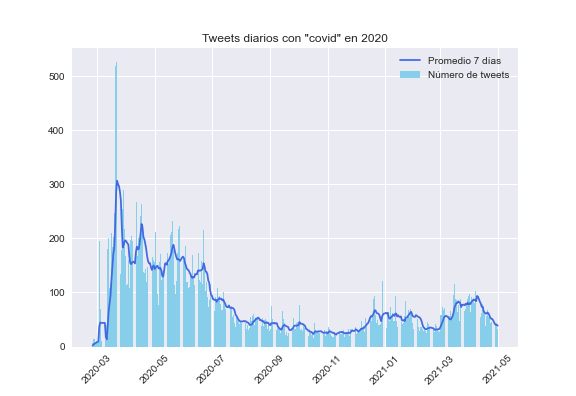
\includegraphics[width=\textwidth]{../imgs/serie_covid_2020.png}
		\end{minipage}
	}
	\subfloat[]{
		\label{fig: serie_pinera_2020}
		\begin{minipage}{0.45\textwidth}
			\centering
			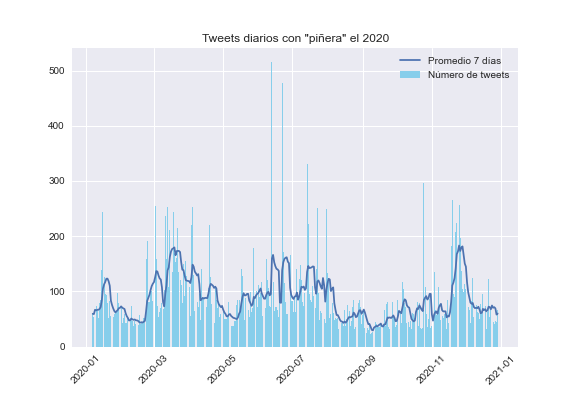
\includegraphics[width=\textwidth]{../imgs/serie_pinera_2020.png}
		\end{minipage}
	}
	\caption{Cantidad de tweets diarios con la palabra \comillas{covid} (izq) y \comillas{piñera} (der).}
\end{figure}

\newpage


En la Figura \ref{fig: serie_covid_2020} vemos que la curva que se genera al suavizar tomando media móvil de siete días es similar a la curva de casos diarios de covid en Chile (también suavizada), pero adelantada en tiempo. El primer peak de los casos diarios ocurrió al rededor de junio \footnote{\href{https://www.google.com/search?client=firefox-b-d&q=covid+chile}{Link a los casos diarios covid en Chile según Google.}}, mientras que en \ref{fig: serie_covid_2020} esto ocurre en marzo cuando todo estaba comenzando. Aproximadamente, en ambas curvas, durante los siguientes seis meses se ve una tendencia a la baja. Esta especie de caracter predictivo de la curva \ref{fig: serie_covid_2020} no es sostenible en el tiempo porque si bien los casos aumentaron hasta superar el primer peak, en Twitter durante enero sólo se ve un aumento relativamente pequeño en la cantidad de tweets asociados al covid. Por otra parte, el peak más alto en \ref{fig: serie_covid_2020} corresponde al día $23$ de marzo del $2020$, en esta fecha se informa la primera muerte por covid en Chile.\\

Con respecto a la Figura \ref{fig: serie_pinera_2020}, observamos que la cantidad de tweets que hablan de Piñera es relativamente constante en el tiempo, con un promedio de $86$ tweets diarios, y sin una tendencia marcada. 
\newpage

\section{Latent Dirichlet Allocation aplicado a datos de Twitter}
	Este algoritmo cae en la categoría del \textbf{Topic Modelling} en la cual se busca, a partir de grandes data sets de texto, encontrar tópicos latentes en estos cosa que sería imposible de hacer humanamente. Para este modelo se necesita un set de palabras $V$ y de tópicos $K$, que sin perdida de generalidad denotamos como $K=\set{1,...,K}$. Los tópicos se modelan como distribuciones de probabilidad sobre el conjunto de palabras $V$. Si bien este algoritmo tiene una fase generativa, su objetivo es calibrar parámetros $\alpha\in [0,1]^{K}$ y $\beta\in[0,1]^{K\times V}$ optimizando cierta cantidad. La idea es, dados $\alpha$ y $\beta$, generar palabras con el siguiente algoritmo:
	
	\begin{itemize}
		\item Se samplea una distribución sobre tópicos $\theta\sim Dir(\alpha, K)$. Notar que $\sum \theta_{i=1}^K = 1$. $Dir$ es la distribución \href{https://en.wikipedia.org/wiki/Dirichlet_distribution}{Dirichlet}.
		\item Dado $\theta$, se samplea un tópico $t\sim\theta$.
		\item Dado el tópico $t$, se samplea una palabra $w\sim\beta_{t\cdot}$.
	\end{itemize}
	
	\begin{remark}
		Este algoritmo nos permite interpretar los parámetros del modelo. $\theta\in\R^{K}$, que sólo depende de $\alpha$, corresponde a que tan relevante es cada tópico. $\beta\in[0,1]^{K\times V}$ modela como se distribuye cada tópico sobre el set de palabras. 
	\end{remark}
	
	Lo anterior permite samplear una $(1)$ palabra y tomamos los sampleos de forma independiente. Consideremos ahora una palabra $w_n$, luego, la probabilidad de generar esta palabra se puede calcular como,
	
	\begin{align*}
		p(w_n|\alpha, \beta) &= \sum_{t\in K} p(w_n|\alpha,\beta,t)p(t|\alpha,\beta)
		= \sum_{t\in K} p(w_n|\beta,t)\int p(t|\alpha,\beta,\theta)p(\theta|\alpha,\beta)d\theta\\
		&= \sum_{t\in K} p(w_n|\beta,t)\int p(t|\theta)p(\theta|\alpha)d\theta.
	\end{align*}
	Donde usamos probabilidades totales y que, según nuestro modelo, $p(w_n|\alpha,\beta,t)=p(w_n|\beta,t)$, $p(t|\alpha,\beta,\theta)=p(t|\theta)$ y $p(\theta|\alpha,\beta)=p(\theta|\alpha)$. Usando la independencia vemos que para $w=(w_1,...,w_N)$,  
	\begin{align*}
		p(w|\alpha,\beta) &= \int p(\theta|\alpha)\parent{\prod_{n=1}^N \sum_{t\in K} p(w_n|t,\beta)p(t|\theta)} d\theta.
	\end{align*}
	
	El calculo anterior tiene razones Bayesianas de ser, esto porque permite calcular la distribución a posteriori de $(\theta, t)$ la cual se busca maximizar. La distribución que se obtiene es intratable numéricamente por lo cual se sigue un approach MCMC o \textbf{variational Bayes}  (\cite{LDA03}, \cite{LDA10}). La implementación de este algoritmo en \texttt{Python} esta dad por la librería \texttt{gensim}\footnote{\href{https://radimrehurek.com/gensim/models/ldamodel.html}{Lda con gensim (link)}}, el código se basa en el script \texttt{onlineldavb.py}\footnote{\href{https://github.com/blei-lab/onlineldavb/blob/master/onlineldavb.py}{Link al repositorio.}} de los autores de \cite{LDA10}. En el citado trabajo, los hiperparámetros cambian un poco asumiendo que la distribución $\beta_{t\cdot}$ de cada tópico $t\in K$ sobre las palabras $V$, es tal que $\beta\sim Dir(\eta, |V|)$. Así, los hiperparámetros (o priors) pasan a ser $(\alpha,\eta)$ y de esta forma son tratados por \texttt{gensim}.\\ 
	
\subsection{Datos}
	Podríamos aplicar el modelo a todos los tweets de cierto espacio y tiempo, pero se decide por otro approach que es trabajar con los tweets de una cuenta en específico dado que el rango de temas o tópicos tocados por una cuenta es menor o más controlado que al trabajar con tweets de muchas cuentas a la vez. La cuenta que se escoge para partir es \texttt{@gabrielboric}, obtenemos sus tweets hasta junio del $2021$. Las características de este data set se pueden apreciar en las Figuras \ref{fig: boric_tweet_año}, \ref{fig: boric_tweet_2020} y \ref{fig: tabla_boric}.

	
	
	
 	\begin{figure}[H]
 		\centering
 		\subfloat[]{
 			\begin{minipage}{0.45\textwidth}
 				\label{fig: boric_tweet_año}
 				\centering
 				\includegraphics[width=\textwidth]{../imgs/boric_tweet_año.png}
 				%\caption{Tweets por año.}
 			\end{minipage}
 		}
 		\subfloat[]{
 			\begin{minipage}{0.45\textwidth}
 				\centering
 				\label{fig: boric_tweet_2020}
 				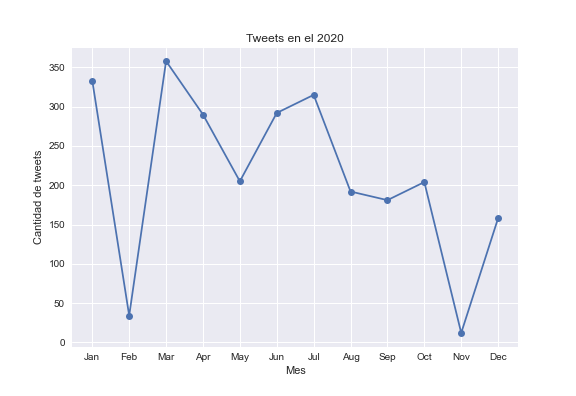
\includegraphics[width=\textwidth]{../imgs/boric_tweet_2020.png}
 				%\caption{Tweets por mes en el año $2020$.}
 			\end{minipage}
 		}
	 	\vfill
	 	\subfloat[]{
	 		\begin{minipage}{0.45\textwidth}
	 			\centering
	 			\label{fig: tabla_boric}
	 			\begin{tabular}{ ||c|c|| } 
	 				\hline
	 				\textbf{Total de tweets} & $39405$ \\ 
	 				\hline
	 				\textbf{Mínimo} & $0$ \\
	 				\hline 
	 				\textbf{Máximo} & $131$ \\
	 				\hline
	 				\textbf{Promedio} & $9.14$ \\
	 				\hline
	 			\end{tabular}
	 		\end{minipage}
	 	}
 		\caption{Tweets por año (a) y por mes en el $2020$ (b). Tamaño del data set y estadísticas de la cantidad diaria de tweets (c).}
 	\end{figure}
	
\subsection{Limpieza y preprocesamiento de datos}
	Los datos que se tienen disponible corresponden a tweets en formato de texto. El procesamiento de base o inicial que se realiza sobre este corpus corresponde a eliminar \textbf{stop words}, links, palabras de largo menor o igual a $3$, caracteres indeseables\footnote{Se eliminaron: \#, comas, signos de exclamación y pregunta, paréntesis y el signo igual.} y finalmente pasar todas las palabras a minúscula. El procesamiento anterior se realizará siempre y al inicio de todo código, luego de este proceso a nivel de vocabulario, se decide eliminar aquellos tweets con una cantidad de palabras menor a $5$ lo que nos deja con $24218$ tweets. Lo siguiente que se puede hacer es quitar palabras de baja frecuencia, sin quitar estas palabras el diccionario\footnote{Entendemos por diccionario al conjunto de todas las palabras utilizadas en el corpus} resultante tiene un tamaño de $35892$ palabras. En el gráfico a continuación muestra la cantidad de palabras resultantes al variar este parámetro.
	
	\begin{figure}[H]
		\centering
		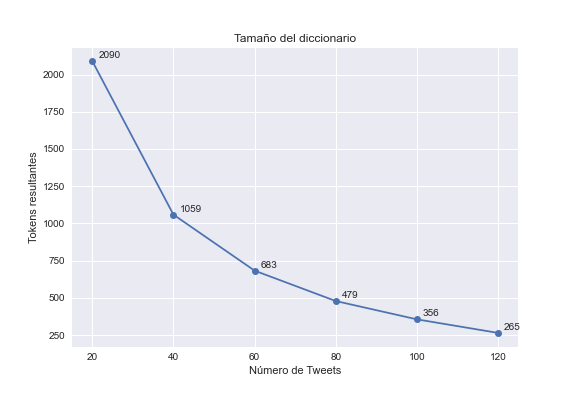
\includegraphics[scale=.5]{../imgs/no_below_len_dict.png}
		\caption{Tamaño del diccionario en función de la cantidad de tweets mínima a la que las palabras deben permanecer. Es decir, $y$ corresponde a las palabras que resultan al filtrar las que aparezcan en menos de $x$ tweets. Este gráfico es importante porque nos permite ver con que tanto vocabulario nos quedamos cuando eliminamos palabras sin mucha importancia o para el modelo.}
	\end{figure}

	

	La siguiente etapa en el preprocesamiento es transformar los tweets en vectores. Para esto, a cada palabra del diccionario, digamos $V$, se le asigna un único índice de forma que el conjunto de palabras (o diccionario) se modela como $\set{1,...,|V|}$. Luego, cada tweet, entendido como una colección de palabras en $V$ de la forma $t=\set{v_1,...,v_n}$, se transforma en $\set{(v_1,r_1),...,(v_n,r_n)}$ donde $v_i$ es el índice de la palabra en $V$ y $r_i$ la cantidad de veces que $v_i$ aparece en $t$. A continuación, un ejemplo de esto.
	
	\begin{figure}[H]
		\centering
		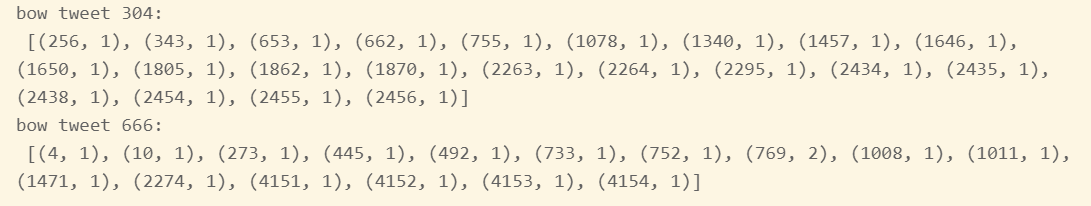
\includegraphics[scale=.5]{../imgs/bow_tweet_informe.png}
		\caption{Estado final de dos tweets escogidos al azar. Esta representación se conoce como \comillas{bow} (\textbf{bag of words}).}
		\label{fig: bow_example}
	\end{figure}
	
	\begin{remark}
		Notar que en los ejemplos que se muestran en la Figura \ref{fig: bow_example}, la segunda componente de las tuplas es mayoritariamente $1$. Esto pasa porque el largo de cada tweet en el corpus es relativamente pequeño en comparación a otros set de datos como por ejemplo una colección de libros o notas periodísticas. Esto sugiere que esta variable no es muy decisiva en este contexto, o bien, que podríamos juntar tweets que estén relativamente cercanos en tiempo, asumiendo que esto implica parentesco temático, para así generar super-tweets de largo mayor. 
	\end{remark}

	\begin{remark}
		Se decide dejar las palabras que hacen referencia a cuentas de Twitter, por ejemplo \texttt{@javier}. La razón de esta decisión es que la aparición de una cuenta en un tópico nos indica que tal persona es relevante para la cuenta sobre la que se está trabajando.
	\end{remark}

	\subsection{Aplicando el modelo}
	Como se comentó en la Sección $2$, para aplicar el modelo usamos la implementación de \texttt{gensim}. El código de la Figura \ref{fig: gensim_code_informe} muestra en términos generales lo necesario para correr el algoritmo sobre nuestro corpus.
	
	\begin{figure}[H]
		\centering
		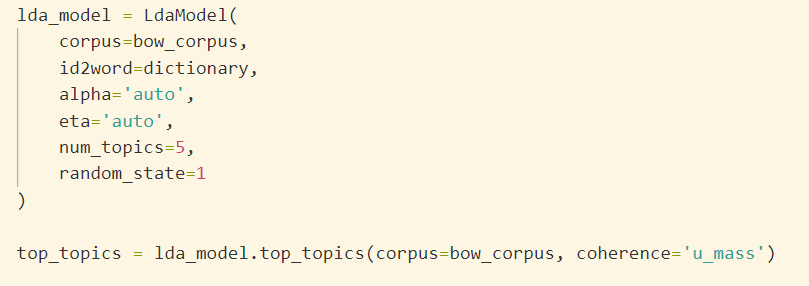
\includegraphics[scale=.4]{../imgs/gensim_code_informe.png}
		\caption{\texttt{corpus} corresponde a lo mostrado en la Figura \ref{fig: bow_example}, \texttt{id2word} es nuestro vocabulario $V$, \texttt{alpha} y \texttt{eta} son los priors discutidos previamente, \texttt{num\_topics} es la cantidad de tópicos que estamos buscando y \texttt{random\_state} es la semilla del algoritmo. El método \texttt{top\_topics} permite obtener coherencia de cada tópico.}
		\label{fig: gensim_code_informe}
	\end{figure}
	El parámetro $\alpha$ lo podemos entregar como \texttt{symmetric}, si queremos que sea un vector, calculado internamente, con todas sus componentes iguales, \texttt{asymmetric}, si queremos que sea un vector como el anterior salvo que sus componentes son distintas, \texttt{auto} si queremos que el algoritmo calcule un vector tipo \texttt{asymmetric} internamente y un escalar $x$ si queremos que sea tipo \texttt{symmetric} pero que el valor que se repita sea $x$. Por otro lado, $\eta$ puede ser todo lo anterior salvo \texttt{asymmetric}. Acá es importante mencionar que el campo \texttt{coherence} del método \texttt{top\_topics} admite las métricas denominadas: \texttt{u\_mass}, \texttt{c\_v}, \texttt{c\_uci} y \texttt{c\_npmi}. De estas, la única que se pudo implementar sin problemas fue \texttt{u\_mass}, el resto arrojaba un error de \texttt{Python} tipo \texttt{Broken Pipe} que no pudo ser solucionado en este proyecto.
	
	\subsubsection{Primera iteración}
	 En la Figura \ref{fig: boric0_informe} se muestra el output de pedirle los tópicos al modelo. En esta primera iteración no estamos filtrando palabras de baja frecuencia y los hiperparámetros $(\alpha, \eta)$ se dejan en default y pedimos $5$ tópicos. 
	
	\begin{figure}[H]
		\centering
		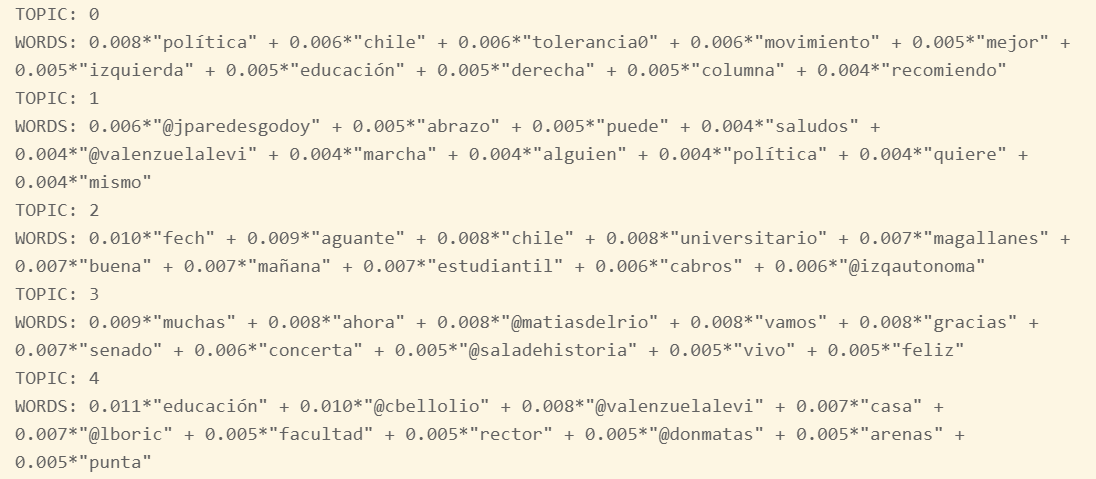
\includegraphics[scale=.4]{../imgs/boric0_informe.png}
		\caption{Los tópicos están ordenados por coherencia y los números que aparecen al lado de cada palabra corresponde a la probabilidad de tal palabra en el tópico. Notar que sólo se muestran las $10$ palabras con mayor probabilidad dentro del tópico, y dado el tamaño de $V$ en este experimento, tales probabilidades son relativamente pequeñas. La coherencia promedio de los tópicos de esta imagen es $-9.1$.}
		\label{fig: boric0_informe}
	\end{figure}

	\subsubsection{Segunda iteración}
	Lo que corresponde ahora es optimizar la coherencia promedio con respecto a $(\alpha, \eta)$ y \texttt{num\_topics}. En la primera aproximación a esta tarea calculamos la \texttt{u\_mass} sobre la grilla $\set{5,6,7,8,9,10}\times\set{\texttt{auto}, 0.5}\times\set{\texttt{auto}, 0.5}$ lo cual nos genera $24$ puntos, ver Figura \ref{fig: param_optimization0_informe}.
	
	 \begin{figure}[H]
	 	\centering
	 	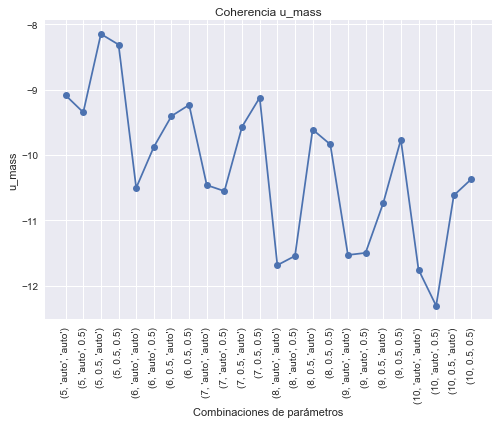
\includegraphics[scale=.4]{../imgs/param_optimization0_informe.png}
	 	\caption{Coherencia por cada combinación de parámetros. Las tuplas del eje $x$ son de la forma $(\texttt{num\_topics}, \alpha, \eta)$.}
	 	\label{fig: param_optimization0_informe}
	 \end{figure}
 	
 	De la Figura \ref{fig: param_optimization0_informe} deducimos que la cantidad de tópicos escogidos es relevante y que mientras menos tópicos fijamos, más será la coherencia promedio. Es por esto que se decide fijar esta variable a $5$ de aquí en adelante. Otra observación es que para número de tópicos fijos $n$, las mejores combinaciones son $(n, 0.5, \texttt{auto})$ y $(n, 0.5, 0.5)$.  

\begin{thebibliography}{99}
	
\end{thebibliography}
\end{document}
